\documentclass[conference]{IEEEtran}
\IEEEoverridecommandlockouts
% The preceding line is only needed to identify funding in the first footnote. If that is unneeded, please comment it out.
\usepackage{soul}
\usepackage{amssymb,amsmath,bm}
\usepackage{graphics,adjustbox}
\usepackage{tikz}
\usepackage{subfigure}
\usepackage{epstopdf}
\epstopdfsetup{suffix={}}
\usepackage{siunitx}
\sisetup{unitsep = \cdot}

\usepackage[figuresright]{rotating}
\usepackage[colorinlistoftodos]{todonotes}
\usepackage[english,algo2e,algoruled,vlined,linesnumbered]{algorithm2e}   % package for algorithm
\usepackage{enumerate}

\usepackage{easyReview}
\newtheorem{assumption}{Assumption}


\DeclareMathOperator*{\argmin}{arg min}

\def\BibTeX{{\rm B\kern-.05em{\sc i\kern-.025em b}\kern-.08em
    T\kern-.1667em\lower.7ex\hbox{E}\kern-.125emX}}
\begin{document}

\title{A Novel Model-Free Actor-Critic  Reinforcement Learning Approach for Dynamic Target Tracking  
%  
% \thanks{This work was supported in part by the Bradley University’s Caterpillar fellowship grant.}
}

\author{%~
  ~ % Author names removed for blind review 
% \IEEEauthorblockN{Amr Elhussein and Md Suruz Miah}
% \IEEEauthorblockA{\textit{Electrical \& Computer Eng.} \\
% \textit{Bradley University}, Peoria, Illinois, USA \\
%  aelhussein@mail.bradley.edu and smiah@bradley.edu}
}

\maketitle

\begin{abstract}
  %
  Addressing the trajectory tracking problem of a mobile robot in tracking a
  dynamic target is still one of the challenging problems in the field of
  robotics. In this paper, we address the position tracking problem of a mobile
  robot where it is supposed to track the position of an mobile target whose
  dynamics is unknown a priori. This problem is even more challenging when the
  dynamics of the mobile robot is also assumed to be unknown, which is indeed a
  realistic assumption. Most of the trajectory tracking solutions proposed in the
  literature in the field of mobile robotics are either focused on algorithms
  that rely on mathematical models of the robots or driven by a overwhelming
  degree of computational complexity. This paper proposes a model-free
  actor-critic reinforcement learning strategy to determine appropriate actuator
  commands for the robot to track the position of the target. We emphasize that
  mathematical models of both mobile robot and the target are not required in
  the current approach. Moreover, Bellman's principle of optimality is utilized
  to minimize the energy required for the robot to track the target. The
  performance of the proposed actor-critic reinforcement learning approach is
  backed by a set of computer experiments with various complexities using a
  virtual circular-shaped mobile robot and a point target modeled by an
  integrator.
%
\end{abstract}

\begin{IEEEkeywords}
  Mobile robots, policy iteration, reinforcement learning, target tracking, trajectory tracking
\end{IEEEkeywords}

% \begin{nomenclature}
% \begin{deflist}[A]
% \defitem{ADP} \defterm{Approximate dynamic programming}
% \defitem{AL}\defterm{Approximate linearization}
% \defitem{RL}\defterm{Reinforcement learning}
% \end{deflist}
% \end{nomenclature}

\section{Introduction}
\label{sec:introduction}


Tracking a random moving target using a mobile robot is a key problem and a
fundamental feature in autonomous robots operating in areas such as
surveillance, search and rescue missions, environmental monitoring, household
cleaning, to name a
few~\cite{kolling2006,Encarnacao2001,Ju2001,Kitowski2012,Zhang2013}. Throughout
the years, the dynamic target tracking problem has received a profound amount of
research in academia and industry \cite{wei2018,liu2019}. This is mainly due to
their inherent complex nonlinear dynamics. Most of the target tracking
algorithms proposed in the literature either rely on A) mathematical and
kinematic models of both the robot and the target~\cite{Huang2008}, B) 
assumption that the target or its trajectory are static and known a priori, and
C) nonlinear control or soft-computing techniques that are driven by large
amount of mostly off-line data that leads to an overwhelming degree of
computational complexity~\cite{KD2007,Cren2017}. In a typical tracking problem,
a robot is to apply a local control actions that enable it to maintain a
relative position and orientation from the designated target while following a
certain trajectory. It can also be applied on a fleet of robots where multiple
robots maintain a geometric configuration relative to the
target\cite{Oh2015-Survey,Liu2017-Modular}.

%Tracking a random moving target using a mobile robot, for instance, is a challenging task.


%Over the past years mobile robots has been used in several applications in commercial and military sectors such as surveillance, search and rescue missions,coverage optimization, cooperative localization and dynamic target tracking tasks to name a few .  In all of these mentioned applications a fleet of robot i.e agents interact with each other to achieve a certain goal. Leader-Follower or dynamic target tracking problem has recieved an extensive amount of study and research in the world of cooperative control theory due to it's promising applications in research and industry. In a typical target tracking formation a number of robots referred to as followers apply local control actions to follow a target in a specific predefined path such as \hl {cyclic, circular motion and time varying communication topologies.} 

Reinforcement learning (RL) is an emerging sub-field of machine learning which
refers to a set of algorithms and techniques in which agents learn by
interacting with the environment and determine their own sets of actions that
define trajectories. Reinforcement learning has long been applied on games and
simulated environments but it has recently been explored to robots in real world
applications, such as localization and mapping, area coverage, path planning and
obstacle avoidance
\cite{kober2013reinforcement,smart2002,michels2005,adekunle2016}.

In this paper, we develop a model-free actor-critic learning approach to control
a non-holonomic wheeled mobile robot. The proposed method offers many advantages
over other methods mentioned in the literature, such as being completely model
free and does not require any knowledge of the mathematical model of the robot
or the moving target and without the need for large computational power. The
steering angle and the linear speed of the robot referred to as the policy
(control actions) are determined by collecting the position and orientation of
both the target and the robot. This set of information is gathered online over a
finite period of time. The optimal control actions are then generated by
utilizing Bellman's principle of optimality which acts as model-free reinforcement learning approach that allows the robot to follow the
trajectory of the target while avoiding collision by maintaining a safe
distance. Here, we extend the work proposed by authors in~\cite{miah2020} by
incorporating actor neural network along with critic network to find optimal
control policy for the trajectory tracking problem. This work acts as the first
milestone in generalizing the algorithm to solve more sophisticated problem such
as typical area coverage and mapping problems in the field of robotics.

The rest of the paper is organized as follows. Section~\ref{sec:problemSetting}
lays down the problem setting of the dynamic target tracking problem and
mathematical models of the robot and the state error. The model~free
actor-critic reinforcement learning algorithm and its associated  mathematical
derivations are detailed in section~\ref{sec:RLSolution}.
Section~\ref{sec:resultsExperiments} illustrates computer experiments for different scenarios that reflect the effectiveness of the proposed method followed by conclusion and future work presented in section~\ref{sec:conclusion}.      

\section{Problem Setting} 
\label{sec:problemSetting}

Fig.~\ref{fig:leaderFollowerSetup} shows the setup of the problem that we address in this manuscript. The robot is characterized by its 2D position $(x_k,y_k)$ and orientation $\theta_k\in[-\pi,\pi)$ with respect to the global coordinate frame X-Y at discrete time index $k=0,1,\ldots,$ where time $t=kT$ with $T>0$ being the sampling time. The time-varying position of the target is denoted by the position vector ${\bf p}_k^{[d]}= [x_k^{[d]},y_k^{[d]}]^T\in\mathbb{R}^2.$  Let the position and orientation (pose) of the robot is denoted by the vector  ${\bf q}_k^T\equiv[x_k,y_k,\theta_k]\in\mathbb{R}^2\times\mathbb{S}^1.$ Without loss of generality, assume that the robot tracks the target trajectory while maintaining line-of-sight distance (also known as the safe distance between the robot and the target) $d>0.$ We emphasize that the mathematical models of both robot and the target are not required in the proposed control technology. For illustration, let us assume that the robot (rear-wheel drive) follows the discrete-time kinematic model described by %
%
\begin{subequations}
  \label{eq:robotModelDT}  
  \begin{align}
    x_{k+1} &= x_k +T\nu_k\cos\theta_k,\\
    y_{k+1} &= y_k +T\nu_k\sin\theta_k,\\
    \theta_{k+1} &= \theta_k + T\frac{\nu_k}{L}\tan\gamma_k,
  \end{align}
\end{subequations}
%
where $\gamma_k\in(-\frac{\pi}{2},\frac{\pi}{2})$ is the steering angle of the font wheel/castor of the robot (see Fig.~\ref{fig:leaderFollowerSetup}), and $\nu_k\in\mathbb{R}$ is the linear speed. Without loss of generality, this work considers a target modeled by an integrator. The discrete-time kinematic model of the target is given as %
%
 \begin{align}
   \label{eq:leaderDT}
   \mathbf{p}_{k+1}^{[d]} = \mathbf{p}_k^{[d]} + T_s \, \mathbf{u}_k^{[d]},
 \end{align}
% 
 with $\mathbf{u}_k^{[d]}\in\mathbb{R}^2$ being the control input vector (velocity) that defines the trajectory (considered random in this work) of the target.  In case, the robot modeled by~\eqref{eq:robotModelDT} is described by a differential drive mobile robot, then its left-wheel velocity $\nu_{L,k}$ and right-wheel velocity $\nu_{R,k}$ are related by
 %
  \begin{figure}
   \centering
   \fcolorbox{gray!10}{gray!5}{
     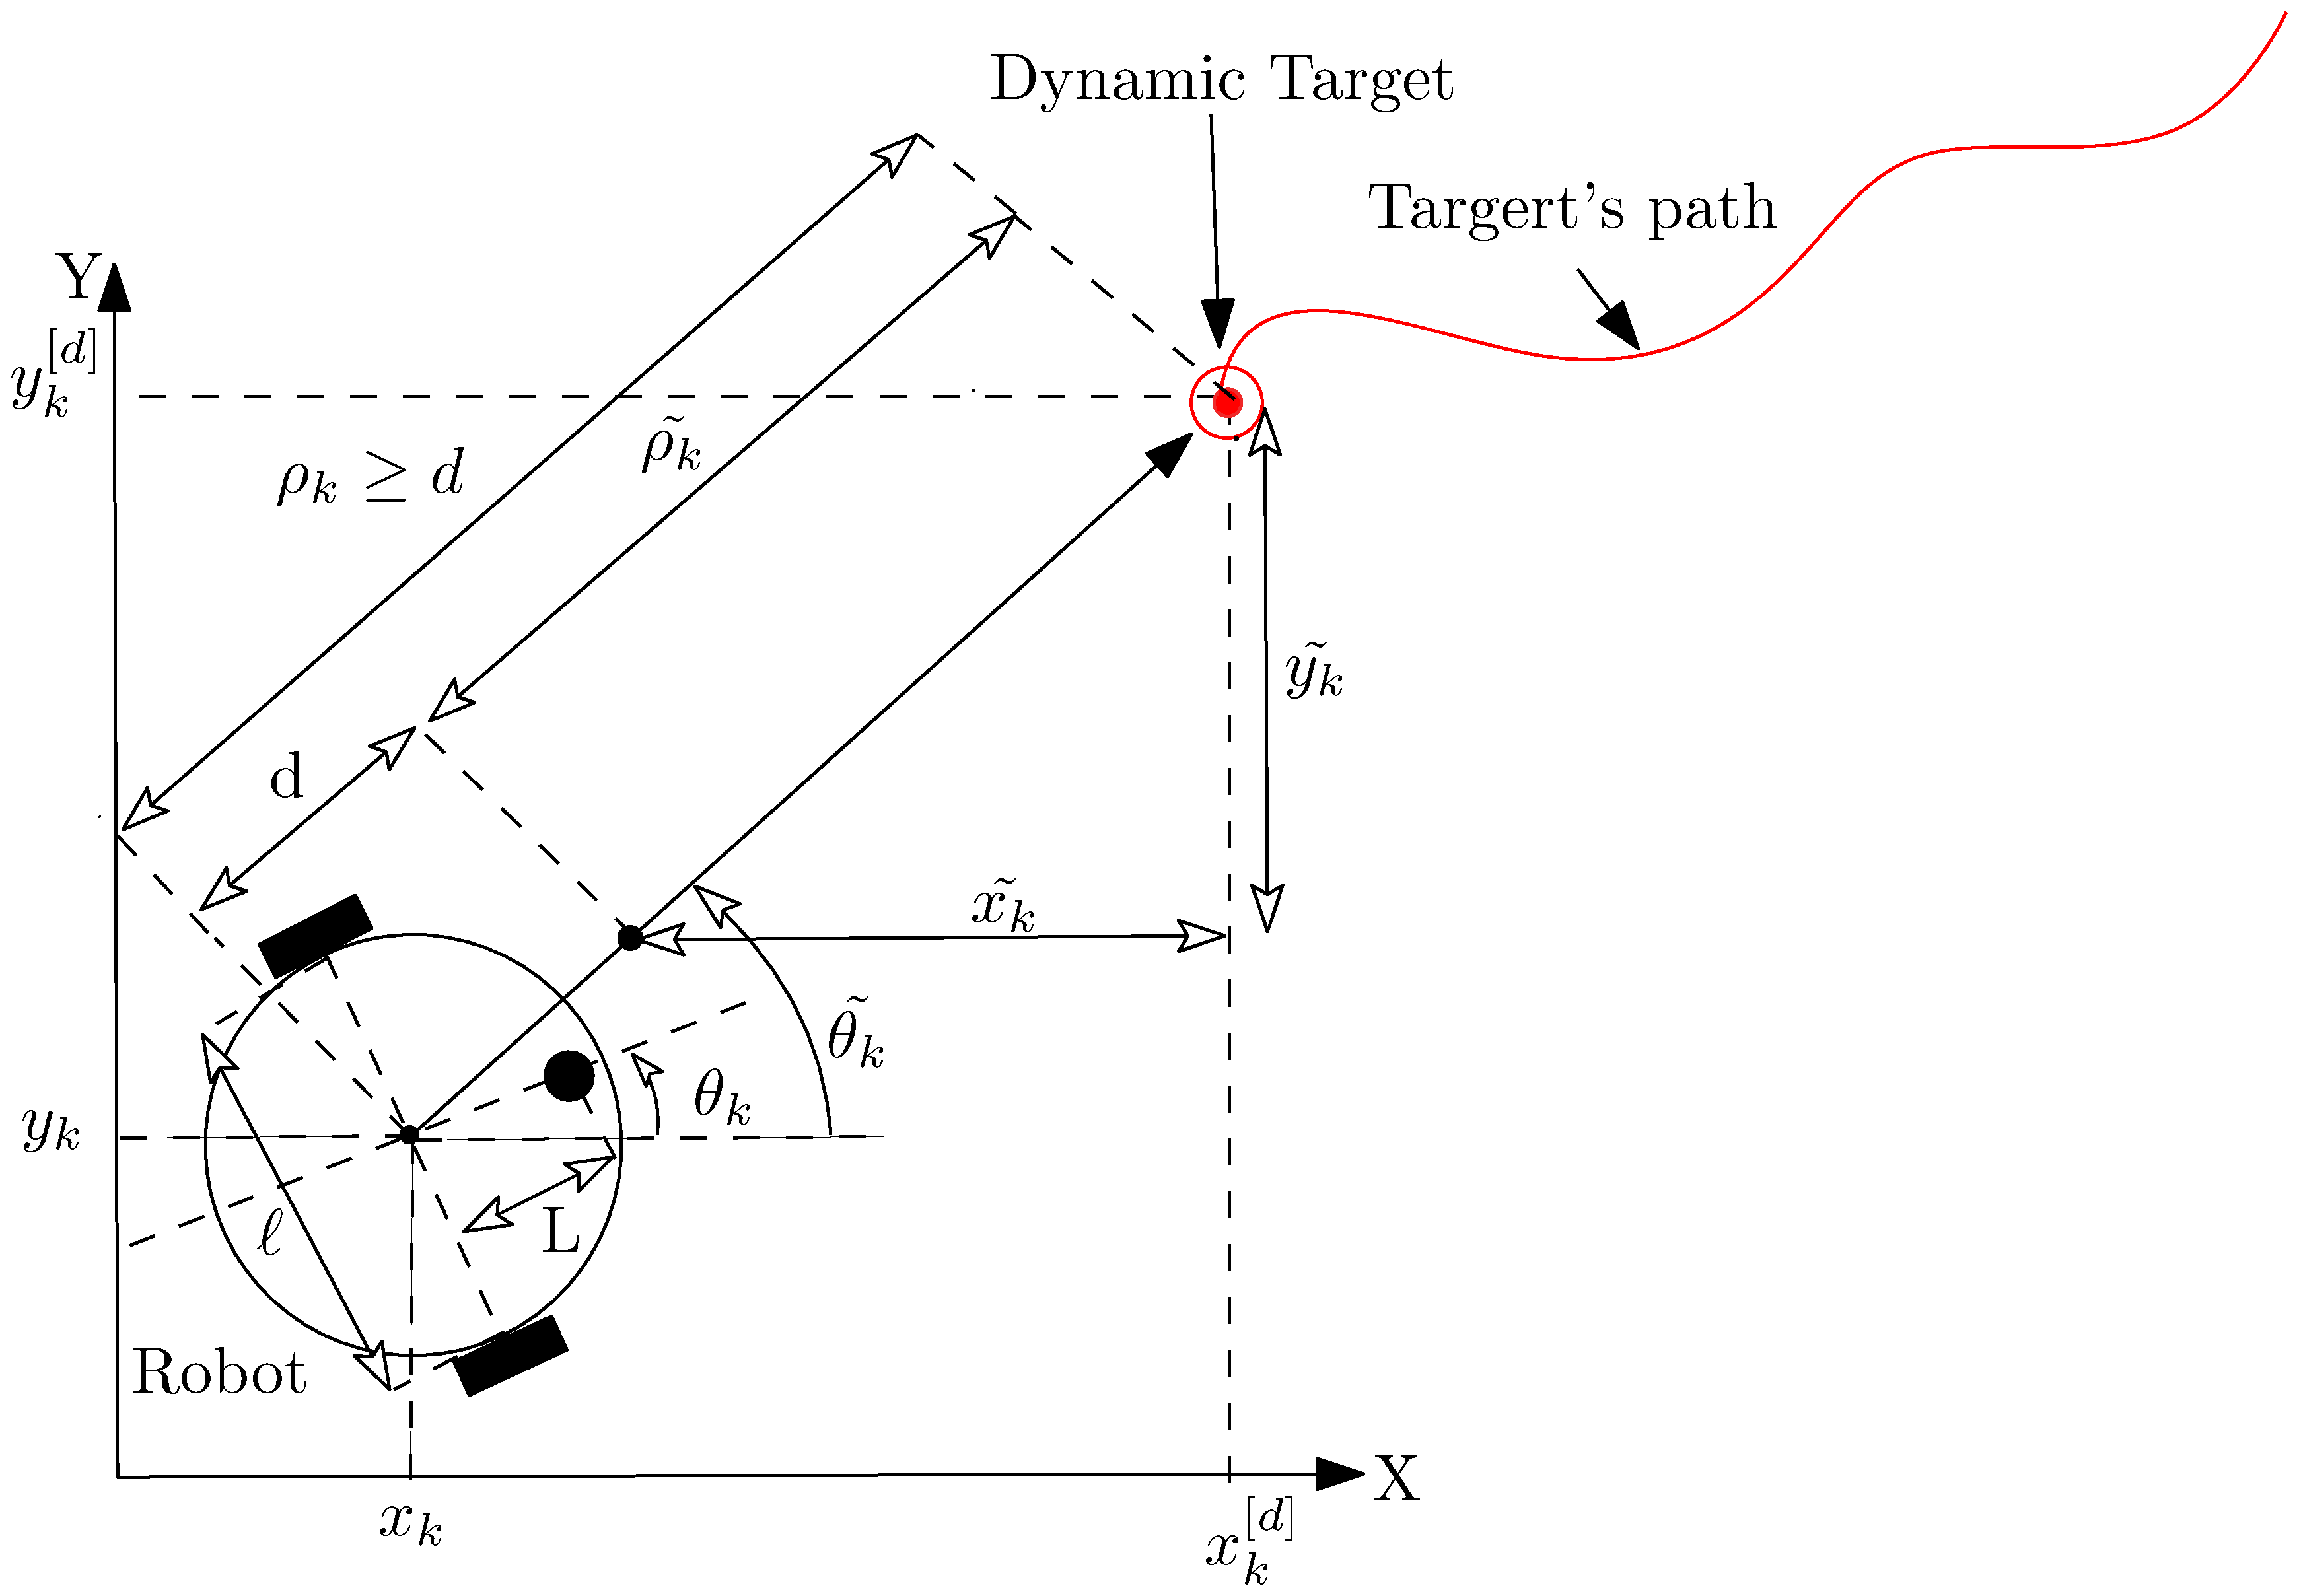
\includegraphics[width=0.45\textwidth]{figs/ipe/LFMICSetup.eps}
    }
   \caption{Mobile robot and its dynamic target tracking problem setup.}
   \label{fig:leaderFollowerSetup}
 \end{figure}
 %
 \begin{subequations}
   \begin{align}
     \nu_{k} &= \frac{1}{2}(\nu_{R,k} + \nu_{L,k}),\\
     \omega_{k} &= \frac{1}{\ell}(\nu_{R,k} - \nu_{L,k}) = \frac{\nu_{k}}{L}\tan(\gamma_k) 	
   \end{align}
 \label{eq:robotModel1-DT}
 \end{subequations}
 %
 where $\omega_k = \frac{\nu_k}{L}\tan\gamma_k$ is the angular velocity of the robot's center $(x_k,y_k).$ Let us define the error vector as 
 \begin{align}
     \label{eq:stateError}
   \mathbf{e}_k = \left[ \tilde{\rho_k},\tilde\theta_k \right]^T=\left[ \sqrt{\tilde{x}_k^2+\tilde{y}_k^2},\tilde{\theta_k} \right]^T% = \\
   % \begin{bmatrix}
   %   \sqrt{(x_k^{[d]} - x_k - d\cos\theta_k^{'})^2+
   %   (y_k^{[d]} - y_k - d\sin\theta_k^{'})^2},
   %   \theta_k^{'} - \theta_k
   % \end{bmatrix},
 \end{align}
% 
 where $\theta_k^{'} = \mathrm{atan2}\left(y_k^{[d]}-y_k, x_k^{[d]}-x_k\right)$
 and $\tilde{\rho}_k =\sqrt{\tilde{x}_k^2+\tilde{y}_k^2} $ is the Euclidean distance (position error) at time instant $k$ as shown in Fig.~\ref{fig:leaderFollowerSetup} with $\tilde{x}_k = x_k^{[d]} - x_k - d\cos\theta_k^{'},$ $\tilde{y}_k = y_k^{[d]} - y_k - d\sin\theta_k^{'},$ and $\tilde{\theta}_k = \theta_k^{'} - \theta_k$ is the orientation error.  The control problem can then be formally stated as follows: Find $\nu_k$ and $\gamma_k$ such that ${\bf e}_k\to {\bf 0}$ as  $k\to\infty$ subject to~\eqref{eq:robotModelDT}~and~\eqref{eq:leaderDT}.

%
%
%  In the next section, a conventional trajectory tracking method is investigated to solve the problem~\eqref{eq:problem}. This is followed by the proposed approximate dynamic programming technique which is illustrated in section~\ref{sec:solutionADP}.




\section{Model-Free Reinforcement Learning Approach}
 \label{sec:RLSolution}

 Reinforcement learning is a promising machine learning technique that is widely
 used for solving problems of many cyber-physical systems that pertain to  
 goal-directed learning from interaction~\cite{sutton2020reinforcement}. In this
 paper, tracking a mobile target using a wheeled mobile robot is formulated as a
 reinforcement learning problem, where the goal of the robot is to track the
 trajectory of a target while maintaining the safe-distance $d>0.$ The RL
 solution employed in the current problem leverages Bellman's principle of
 optimality to decide on the appropriate control actions (actuator commands) for
 the robot to track the position trajectory of the target. The relative
 importance of the states in the error vector ${\bf e}_k$ and the control
 decisions (linear velocity $\nu_k$ and steering angle $\gamma_k$) of the robot
 are evaluated using the performance (cost) index %
 %
 \begin{align}
 \label{eq:costFunctional}
   J =  \frac{1}{2} \sum_{k=0}^\infty\left[{\bf e}_k^T \, {\bf Q} \, {\bf e}_k + {\bf u}_k^T \, {\bf R} \, {\bf u_k}\right],
 \end{align}
 %
 where ${\bf Q}\in\mathbb{R}^{2\times 2}$ and ${\bf R}\in\mathbb{R}^{2\times 2}$ are symmetric positive definite weighting matrices, and ${\bf u}_k^T = [\nu_k,\gamma_k]$ is the control input vector.  The objective of the optimization problem, following~\cite{Lewis2013-Reinforcement}, is to find an optimal sequence of control polices $\{\mathbf{u}^*_k\}_{k=0}^\infty$ that minimizes the cost index $J$ along the state-trajectories~\eqref{eq:leaderDT}~and~\eqref{eq:robotModelDT}. Motivated by the structure of the convex quadratic cost functional~\eqref{eq:costFunctional}, let the solution of the tracking control problem employ the value function $V({\bf e}_k,{\bf u}_k)$ defined by %
 %
 \begin{equation*}
 \label{eq:valueFunction}
 V({\bf e}_k,{\bf u}_k) = \sum_{\kappa=k}^\infty \frac{1}{2}\left({\bf e}_\kappa^T\, {\bf Q}\, {\bf e}_\kappa + {\bf u}_\kappa^T \, {\bf R}\, {\bf u_\kappa}\right).
 \end{equation*}
 %
 This structure yields a temporal difference form (i.e., Bellman equation) as follows
 \begin{equation*}
 \label{eq:tempraldiffeq}
 V({\bf e}_k,{\bf u}_k)= \frac{1}{2}\left[{\bf e}_k^T\, {\bf Q}\, {\bf e}_k + {\bf u}_k^T\, {\bf R}\, {\bf u_k}\right] +V({\bf e}_{k+1},{\bf u}_{k+1}).
 \end{equation*}
 %
 Bellman's optimality principle yields the optimal control policies ${\bf u}_k^*,~k\ge 0,$ such that~\cite{Lewis2012} %
 %
 \begin{align*}
   {\bf u}^*_k = \argmin_{{\bf u}_k}\left[\frac{1}{2}\left[{\bf e}^T_k\,  {\bf Q}\, {\bf e}_k +{\bf u}^T_k\,  {\bf R} \,  {\bf u}_k\right]   +
   V^*({\bf e}_{k+1},{\bf u}_{k+1}^*)\right].
   \label{eq:argMinControlAction}
 \end{align*}
 %
 Alternatively, this optimal  policy form is equivalent to ${\bf u}^*_k = \argmin_{{\bf u}_k}\left[
 V({\bf e}_{k},{\bf u}_{k})\right].$ 
 Therefore, the underlying Bellman optimality equation follows %
 %
 \begin{equation*}
 \label{eq:BellOpt}
 V^*({\bf e}_k,{\bf u}^*_k)= \frac{1}{2}\left[{\bf e}_k^T\, {\bf Q}\, {\bf e}_k + {\bf u}_k^{*T}\, {\bf R}\, {\bf u}^*_k\right] +V^*({\bf e}_{k+1},{\bf u}^*_{k+1}),
 \end{equation*}
 %
 where $V^*(\cdot,\cdot)$ is the optimal solution for Bellman's optimality equation. This temporal difference equation is utilized by reinforcement learning process which solves the following temporal difference approximation form %
 %
 \begin{align}
   V(\mathbf{z}_k) = \frac{1}{2}\mathbf{z}_k^T\, \bar{\mathbf{P}}\, \mathbf{z}_k + V(\mathbf{z}_{k+1}),
 \label{eq:valueFunctionEstimated}
 \end{align}
 %
 where $\mathbf{z}_k = \left[\mathbf{e}_k ,\mathbf{u}_k\right]^T\in\mathbb{R}^4,$ $V\left(\mathbf{e}_k,\mathbf{u}_k\right) \equiv V(\mathbf{z}_k),$  and $\bar{\mathbf{P}}$ is a symmetric block-diagonal matrix formed using $(\mathbf{Q},\mathbf{R}),$~\textit{i.e.,~}$\bar{\mathbf{P}} = \mathrm{blockdiag}(\mathbf{Q},\mathbf{R}).$ %
 The approximation of the solving value function $V(\mathbf{z}_k)$ employs a quadratic form so that $\hat{V}(\mathbf{z}_k)=\frac{1}{2}\mathbf{z}_k^T\, \mathbf{P}\, \mathbf{z}_k,$ for some positive definite matrix  $\mathbf{P}\in\mathbb{R}^{4\times 4}.$ The optimal control input ${\bf u}_k^*$ is then determined by setting $\frac{\partial\hat{V}({\bf z}_k)}{\partial{\bf u}_k} = 0,$ which yields %
 %
 \begin{align}
 \label{eq:modelFreePolicy}    
 \mathbf{u}_k^* = -\,  \mathbf{P}_{uu}^{-1}\, \mathbf{P}_{ue}\, \mathbf{e}_k,
 \end{align}
 %
 where $\mathbf{P}_{uu}$ and $\mathbf{P}_{ue}$ are sub-blocks of symmetric matrix $\mathbf{P}.$ The proposed approach approximates the block matrix ${\bf P}$ by following a two-step solution mechanism based on policy iteration method~\cite{sutton2020reinforcement}, which in turn approximates the value function~$V(\cdot).$ First, a multi-layer critic neural network shown in Fig.~\ref{fig:nnCritic} is used for determining the estimated value function, $\hat V({\bf z}_k).$
\begin{figure}
    \centering
    \fcolorbox{blue}{gray!5}{
        \begin{adjustbox}{max width = 0.45\textwidth}
            \tikzset{%
                input neuron/.style={
                    circle,
                    fill=green!50,
                    minimum size=0.7cm
                },
                neuron missing/.style={
                    draw=none, 
                    scale=1,
                    fill=white,
                    text height=0.01cm,
                    execute at begin node=\color{black}$\vdots$
                },
            }
           
            \tikzset{%
                hidden neuron/.style={
                    circle,
                    fill=blue!50,
                    minimum size=0.7cm
                },
                neuron missing/.style={
                    draw=none, 
                    scale=1,
                    fill=white,
                    text height=0.01cm,
                    execute at begin node=\color{black}$\vdots$
                },
            }
           
            \tikzset{%
                output neuron/.style={
                    circle,
                    fill=red!50,
                    minimum size=0.7cm
                },
                neuron missing/.style={
                    draw=none, 
                    scale=1,
                    fill=white,
                    text height=0.01cm,
                    execute at begin node=\color{black}$\vdots$
                },
            }
           
            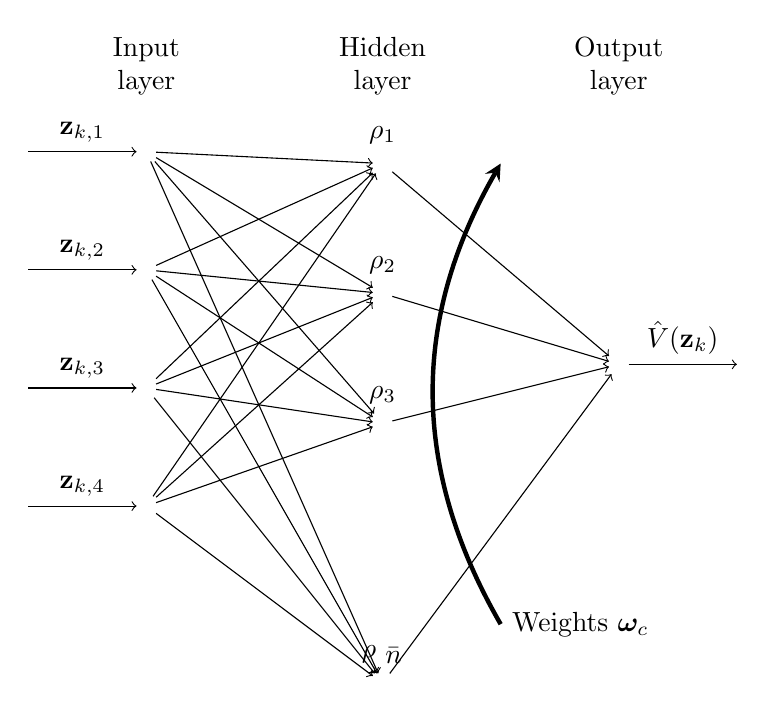
\begin{tikzpicture}[x=1.5cm, y=1.5cm]
           
            \foreach \m/\l [count=\y] in {1,2,3,4}
            \node [input neuron/.try, neuron \m/.try] (input-\m) at (0,2.5-\y) {};
           
            \foreach \m [count=\y] in {1,2,3,missing,4}
            \node [hidden neuron/.try, neuron \m/.try ] (hidden-\m) at (2,2.5-\y*1.1) {};
           
            \foreach \m [count=\y] in {1}
            \node [output neuron/.try, neuron \m/.try] (output-\m) at (4,2.5-\y*2.8) {};
           
            \foreach \l [count=\i] in {1,2,3,4}
            \draw [<-] (input-\i) -- ++(-1,0)
            node [above, midway] {$\mathbf{z}_{k,\l}$};
           
            \foreach \l [count=\i] in {1,2,3,~\mbox{$\bar{n}$}}
            \node [above] at (hidden-\i.north) {$\rho_{\l}$};
           
            \foreach \l [count=\i] in {1}
            \draw [->] (output-\i) -- ++(1,0)
            node [above, midway] {$\hat{V}(\mathbf{z}_{k})$};
            % node [above, midway] {$\hat{V}_\l$};
           
            \foreach \i in {1,...,4}
            \foreach \j in {1,...,4}
            \draw [->] (input-\i) -- (hidden-\j);
           
            \foreach \i in {1,...,4}
            \foreach \j in {1}
            \draw [->] (hidden-\i) -- (output-\j);
           
           
           
            \foreach \l [count=\x from 0] in {Input, Hidden, Output}
            \node [align=center, above] at (\x*2,1.9) {\l \\ layer};
           
            \draw[-stealth,ultra thick](3,-2.5)node[right]{Weights $\boldsymbol{\omega}_c$} to[bend left] (3,1.4);
           
            \end{tikzpicture}
        \end{adjustbox}      
    }
    \caption{Multi-layer critic neural network for approximating value function $V({\bf z}_k).$}
    \label{fig:nnCritic}
      \end{figure}
 %      
      Second, the policy evaluation step that follows is utilized to update the critic weights $\bm{\omega}_c$ in real-time regardless of the mathematical models of the robot and the target. This step is aimed to search for a strictly better policy using the updated critic weights $\bm{\omega}_c.$ Note that $\hat V({\bf z}_k)$ can also be written using temporal difference form as $\hat V({\bf z}_k) = \mathbf{z}_k^T\, \bar{\mathbf{P}}\, \mathbf{z}_k + \hat V({\bf z}_{k+1}),$ which is described by
 %
 \begin{equation}
 \label{eq:const}
 \mathbf{z}_k^T\, \mathbf{P}\, \mathbf{z}_k - \mathbf{z}_{k+1}^T\, \mathbf{P}\, \mathbf{z}_{k+1} = \mathbf{z}_k^T\, \bar{\mathbf{P}}\, \mathbf{z}_k. 
 \end{equation}
 %
 Equation~\eqref{eq:const} is evaluated repeatedly to collect data online for at least $\eta\ge \bar n,$ with $\bar n= (2+2)(2+2+1)/2 = 10$ evaluation steps due to the fact that the matrix ${\bf P}$ is positive definite and symmetric. The strictly better policy matrix ${\bf P},$ is determined every $\eta$ time/evaluation steps. To find the better policy in terms of matrix ${\bf P},$ let us define the vector $\boldsymbol{\omega}=\mathrm{vec}(\mathbf{P})\in\mathbb{R}^{16},$ which is formed by stacking columns of ${\bf P}$ matrix.  However, since ${\bf P}$ is symmetric, we only need to determine the weight $\bm{\omega}_c\in\mathbb{R}^{\bar n}$ using the critic neural network shown in Fig.~\eqref{fig:nnCritic}. The left hand side of~\eqref{eq:const} is expressed using the following critic approximation form %
 %
 $$\hat{V}(\mathbf{z}_k)-\hat{V}(\mathbf{z}_{k+1})=\boldsymbol{\omega}_c^T\tilde{\bm{\rho}}(\mathbf{z}_{k,k+1}),$$
 %
 where $\tilde{\bm{\rho}}(\mathbf{z}_{k,k+1})=\bm{\rho}(\mathbf{z}_k)-\bm{\rho}(\mathbf{z}_{k+1}) \in \mathbb{R}^{10 \times 1}, \, \bm{\rho}(\mathbf{z}_k)=\left(\mathbf{z}_k\otimes\mathbf{z}_k\right)$, which is a Kronecker product that generates the basis function vector with components $z_{k,1}^2,$ $z_{k,1}z_{k,2},$ $z_{k,1}z_{k,3},$ $z_{k,1}z_{k,4},$ $z_{k,2}^2,$ $z_{k,2}z_{k,3},$ $z_{k,2}z_{k,4},$ $z_{k,3}^2,$ $z_{k,3}z_{k,4},$ and $z_{k,4}^2.$ Note that the critic weight $\bm{\omega}_c$ is related to the policy matrix ${\bf P}$ as  $\boldsymbol{\omega}_c^T = [0.5 \, P^{11},P^{12},P^{13},P^{14},  \, 0.5 \, P^{22}, P^{23},P^{24},$ $\,0.5 \, P^{33}, P^{34},\,0.5 \ P^{44}, ]^T \in \mathbb{R}^{1\times 10}$ with $P^{ij}$ being the $ij^{th}$ entry of matrix $\mathbf{P}.$ %
 %
 Here, the critic weights $\boldsymbol{\omega}_c$ are updated using a gradient descent update rule. The tuning error $\varepsilon_k$ at each computational instance $k$ is given by $\varepsilon_k =\boldsymbol{\omega}_c^T\tilde{\bm{\rho}}(\mathbf{z}_{k,k+1})-{v}_k,$ where $v_\kappa = \frac{1}{2}\mathbf{z}_{k}^T \, \bar{\mathbf{P}} \, \mathbf{z}_{k}$. The error data $\varepsilon_k$ is collected online for at least  $\eta \ge \bar n$ evaluation steps before updating the critic weights $\boldsymbol{\omega}_c$ that is used to determine the improved policy matrix ${\bf P}.$ The sum of squared tuning errors is given by 
 %
 \begin{align}
   \delta_c =\frac{1}{2}\sum_{\kappa=0}^{\eta-1}\varepsilon_{k+\kappa}^2 &=\frac{1}{2}\sum_{\kappa=0}^{\eta-1}(\boldsymbol{\omega_c}^T\tilde{\bm{\rho}}(\mathbf{z}_{k+\kappa,k+\kappa+1})-{v}_{k+\kappa})^2 \nonumber \\        	
   	&=\frac{1}{2}\| \mathbf{v} - \bm{\Lambda}\bm{\omega_c}\|^2 \nonumber \\
   &=\frac{1}{2}\left(\mathbf{v} - \bm{\Lambda}\bm{\omega_c}\right)^T \left(\mathbf{v} - \bm{\Lambda}\bm{\omega_c}\right), 
 \end{align}
 where $\bm{\Lambda} = [{\bf o}_0,{\bf o}_1,\ldots,{\bf o}_{\eta-1}]^T \in \mathbb{R}^{\eta\times 10}$ with ${\bf o}_\kappa = \tilde{\bm{\rho}}^T({\bf z}_{k+\kappa, k+\kappa+1}) \in \mathbb{R}^{1\times 10}$ and ${\bf v} =[v_0,v_1,\ldots,v_{\eta-1}]^T \in \mathbb{R}^{\eta}$ with $v_\kappa = \frac{1}{2}\mathbf{z}_{k+\kappa}^T \, \bar{\mathbf{P}} \, \mathbf{z}_{k+\kappa}$ for $\kappa = 0,1,\ldots, \eta-1$. %
 The sum of squared error $\delta_c$ can be minimized by adapting the critic weight using the gradient decent approach for at least $\bar n$ data samples as 
 \begin{multline}
   \bm{\omega}_c^{[r+1]} = \bm{\omega}_c^{[r]} - \ell_c\frac{\partial\delta_c}{\partial \bm{\omega_c}} = \bm{\omega}_c^{[r]} - \ell_c\left(-\bm{\Lambda}^T\mathbf{v} + \bm{\Lambda}^T \bm{\Lambda}\bm{\omega}_c^{[r]}\right)\\ 
 =\bm{\omega}_c^{[r]} - \ell_c \bm{\Lambda}^T\left(\bm{\Lambda}\bm{\omega}_c^{[r]}-\mathbf{v}\right), 
 \label{eq:criticWeights}
 \end{multline}
 %
 where $0<\ell_c<1$ is a critic learning rate and $r$ is known as iteration index for updating the policy. The updated critic weights can be used to reconstruct the policy matrix ${\bf P}$ as
 
 \begin{center}
 ${\bf P}=\begin{bmatrix} 
 2\,\omega_c^{[1]}    & \omega_c^{[2]}      & \omega_c^{[3]}       & \omega_c^{[4]}        \\ 
 \omega_c^{[2]}       &2\, \omega_c^{[5]}   & \omega_c^{[6]}       & \omega_c^{[7]}        \\
 \omega_c^{[3]}       & \omega_c^{[6]}      &2\, \omega_c^{[8]}   & \omega_c^{[9]}   \\   
 \omega_c^{[4]}       & \omega_c^{[7]}      & \omega_c^{[9]}      & 2\,\omega_c^{[10]}      
 \end{bmatrix}\in \mathbb{R}^{4\times 4},$
 \end{center}
 %
 where $\omega^{[i]}$ is the $i^{th}$ entry of the weight vector $\bm{\omega}_c.$ 

 The critic weights are then used to update the actor weights $W_a\in\mathbb{R}^{n\times m}$ (here $n=2$ and $m=2$) which maps the state error to the desired policy (control actions) at time step $k$ with the following equation:
 \begin{align}
 \label{eq:actorWeightsPolicy}    
 \hat{\mathbf{u}}_k  =  {\bf W}_a^T \bm{\sigma}(\mathbf{e}_k),
 \end{align}
 %
 where ${\bf W}_a\in\mathbb{R}^{n^{'}\times 2}$ is the actor weight matrix and $\bm{\sigma}:\mathbb{R}^2 \to \mathbb{R}^{n^{'}}$ is the basis function vector.  Equation~\eqref{eq:actorWeightsPolicy} is realized using a multi-layer actor neural network shown in Fig.~\ref{fig:nnActor}. %
 %
\begin{figure}
  \centering
  \boxed{
    \begin{adjustbox}{max width = 0.48\textwidth}
      \tikzset{%
        input neuron/.style={
          circle,
          fill=green!50,
          minimum size=0.7cm
        },
        neuron missing/.style={
          draw=none, 
          scale=1,
          fill=white,
          text height=0.01cm,
          execute at begin node=\color{black}$\vdots$
        },
      }

      \tikzset{%
        hidden neuron/.style={
          circle,
          fill=blue!50,
          minimum size=0.7cm
        },
        neuron missing/.style={
          draw=none, 
          scale=1,
          fill=white,
          text height=0.01cm,
          execute at begin node=\color{black}$\vdots$
        },
      }

      \tikzset{%
        output neuron/.style={
          circle,
          fill=red!50,
          minimum size=0.7cm
        },
        neuron missing/.style={
          draw=none, 
          scale=1,
          fill=white,
          text height=0.01cm,
          execute at begin node=\color{black}$\vdots$
        },
      }      

      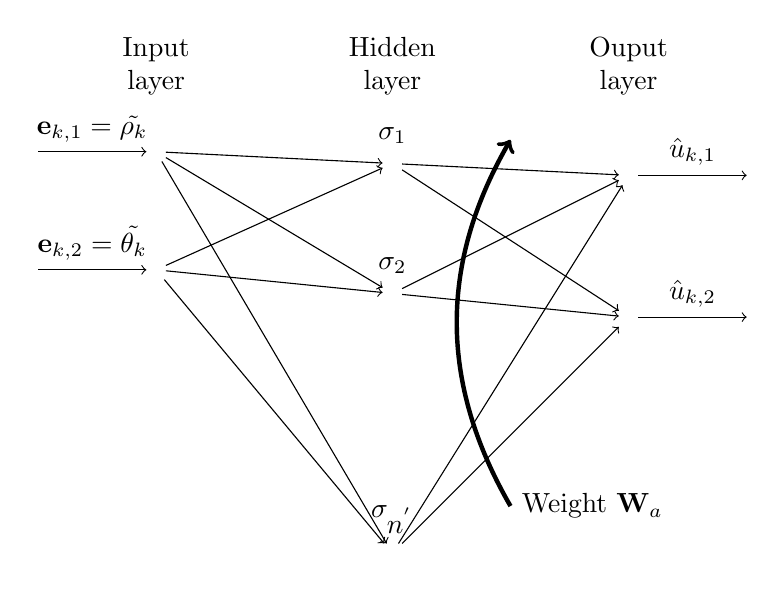
\begin{tikzpicture}[x=1.5cm, y=1.5cm]

        \foreach \m/\l [count=\y] in {1,2}
        \node [input neuron/.try, neuron \m/.try] (input-\m) at (0,2.5-\y) {};

        \foreach \m [count=\y] in {1,2,missing,3}
        \node [hidden neuron/.try, neuron \m/.try ] (hidden-\m) at (2,2.5-\y*1.1) {};

        \foreach \m [count=\y] in {1,2}
        \node [output neuron/.try, neuron \m/.try] (output-\m) at (4,2.5-\y*1.2) {};

        \foreach \l [count=\i] in {1}
        \draw [<-] (input-\i) -- ++(-1,0)
        node [above, midway] {$\mathbf{e}_{k,1}=\tilde{\rho_{k}}$};
        \draw [<-] (input-2) -- ++(-1,0)
        node [above, midway] {$\mathbf{e}_{k,2}=\tilde{\theta_{k}}$};
        \foreach \l [count=\i] in {1,2,\mbox{$n^{'}$}}
        \node [above] at (hidden-\i.north) {$\sigma_{\l}$};

        \foreach \l [count=\i] in {1,2}
        \draw [->] (output-\i) -- ++(1,0)
        node [above, midway] {$\hat{u}_{k,\l}$};

        \foreach \i in {1,...,2}
        \foreach \j in {1,...,3}
        \draw [->] (input-\i) -- (hidden-\j);

        \foreach \i in {1,...,3}
        \foreach \j in {1,2}
        \draw [->] (hidden-\i) -- (output-\j);
        
        \foreach \l [count=\x from 0] in {Input, Hidden, Ouput}
        \node [align=center, above] at (\x*2,1.9) {\l \\ layer};

        \draw[->,ultra thick]
        (3,-1.5)node[anchor=west]{Weight~${\bf W}_a$} to[bend left] (3,1.6);
      \end{tikzpicture}
    \end{adjustbox}      
    }
  \caption{Actor neural network structure for approximating control input.}
  \label{fig:nnActor}
\end{figure}
%
The elements of the vector function $\bm{\sigma}(\cdot)$ are the activation functions of the neurons in the hidden layer shown in Fig.~\ref{fig:nnActor}. We will need to determine the actor weight matrix ${\bf W}_a$ that minimizes the error between the estimated control inputs determined by model~\eqref{eq:actorWeightsPolicy} and that determined by critic neural network approximation model~\eqref{eq:modelFreePolicy}. For that, let us define the error %
%
\begin{align}
  \label{eq:deltaActor}
  \delta_a = \frac{1}{2}\|\hat{{\bf u}}_k - {\bf u}_k^*\|^2,
\end{align}
%
which can be written as %
%
\begin{align*}
  \delta_a = \frac{1}{2}\left( {\bf W}_a^T\bm{\sigma}({\bf e}_k) -  {\bf u}_k^*\right)^T\left( {\bf W}_a^T\bm{\sigma}({\bf e}_k) -  {\bf u}_k^*\right). 
\end{align*}
%
Taking partial derivative of the above expression of $\delta_a$  with respect to ${\bf W}_a$ gives %
%
\begin{multline*}
  \frac{\partial \delta_a}{\partial{\bf W}_a} = \bm{\sigma}({\bf e}_k)\bm{\sigma}^T({\bf e}_k){\bf W}_a - \bm{\sigma}({\bf e}_k)\left( {\bf u}_k^* \right)^T\\
  =\bm{\sigma}({\bf e}_k)\left[ \bm{\sigma}^T({\bf e}_k){\bf W}_a -\left( {\bf u}_k^* \right)^T \right].
\end{multline*}
%
Therefore, actor weight matrix ${\bf W}_a$ in every policy iteration $r = 0,1,2,\ldots$ can be updated using the learning rule %
%
\begin{multline}
  {\bf W}_a^{[r+1]} = {\bf W}_a^{[r]} - \ell_a\frac{\partial\delta_a}{\partial{\bf W}_a}\\
  = {\bf W}_a^{[r]} - \ell_a\bm{\sigma}({\bf e}_k)\left[ \bm{\sigma}^T({\bf e}_k){\bf W}_a -\left( {\bf u}_k^* \right)^T \right], 
 \label{eq:actorWeights}
\end{multline}
%
 where $\ell_a$ is the actor learning rate.  The complete policy iteration
 solution process for the target tracking problem is detailed out in Algorithm~\ref{alg:ModelFreeTracking}. 
 %
 \begin{algorithm2e}{
     \caption{\label{alg:ModelFreeTracking} Model-free actor-critic reinforcement learning using the policy iteration solution.}
     \DontPrintSemicolon
     \KwIn{Sampling-time $T_s,$ $\mathbf{Q},~\text{and}~\mathbf{R}$ }
     \KwOut{Error trajectory $\mathbf{e}_k,$ for $k=0,1,\ldots$}
     % \KwData{Map representation using occupancy grid technique}
     % \KwResult{output******************************}
     \Begin{
         $k=0, r = 0$ \tcc*[h]{Discrete time and policy indices}\;
         n = 2 , m = 2 \tcc*[h]{state error and input dimensions}\;
         $\eta = (n+m)(n+m+1)/2$\;
         Initialize $\mathbf{P}^{[0]}$ \tcc*[h]{Positive definite}\;
                 Set offset distance $d$\;
                 Given approximate initial poses of leader and follower, compute $\mathbf{e}_0$ using error model~\eqref{eq:stateError}\;
                 Compute follower's input $\mathbf{u}_0^{[0]}$ using policy~\eqref{eq:actorWeightsPolicy}\;
         \Repeat(\tcc*[h]{Main timing loop}){Tracking errors are zero}
         {
             Find $\mathbf{e}_{k+1}$ using~\eqref{eq:stateError}\;
             Compute policy $\mathbf{u}_{k+1}^{[r]}$ using~\eqref{eq:actorWeightsPolicy}\;
             %Evaluate and record Equation~\eqref{eq:modelFreeMatrixSolution}\;
             \If{[$(k+1)~\mathrm{modulo}~\eta]==0$ }
             {
                 $r\leftarrow r+1$\tcc*[h]{Evaluate policy}using~\eqref{eq:modelFreePolicy}\;
                 Solve for the critic-weights $\bm{\omega_c}$ using~\eqref{eq:criticWeights}\;
                 Solve for the actor-weights $\bm{\omega_a}$ using ~\eqref{eq:actorWeights}\;
                 Construct matrix $\mathbf{P}^{[r]}$ using vector $\bm{\omega_c}$\;
 %                \eIf{$\|\mathbf{P}^{[r]} - \mathbf{P}^{[r+1]}\|<\varepsilon$}{Set $\mathbf{u}_{k+1}^*\leftarrow\mathbf{u}_{k+1}^{[r]}$}{$k\leftarrow k+1$ }
             }}
 %        {
 %                $k\leftarrow k+1$
 %            }
         $k\leftarrow k+1$
         }
     }
 \end{algorithm2e}    
 %
For clarity, number of hidden neurons chosen in the actor neural network shown in Fig.~\ref{fig:nnActor} is $n^{'} = 2$ and the basis function vector is simply $\bm{\sigma}({\bf e}_k) = {\bf e}_k.$ In the following, we provide the computer simulation results to highlight the performance of the proposed model-free trajectory tracking approach for a mobile robot in tracking a random target while maintaining a geometric safe distance $d>0.$  
    


  

 \section{Computer Experiments and Results}
 \label{sec:resultsExperiments}

 This section adopts the theoretical results discussed in the previous section by simulating Algorithm~\ref{alg:ModelFreeTracking} using a differential drive mobile robot. The proposed actor-critic RL algorithm is tested  utilizing MATLAB software in a laptop computer running Ubuntu 18.04 as a preliminary step to implement the Algorithm experimentally in real world. Here we present the performance of the proposed method and the convergence characteristics of the actor and critic weights. The weighting matrices are set to $\mathbf{Q} = \mathrm{diag}[0.001,0.001]$ and $\mathbf{R} = \mathrm{diag}[10^{-5}, 10^{-5}].$ % 
  % \[Q=0.001 
  % \begin{bmatrix}
  % 1       & 0   \\
  % 0       & 1   \\
  % \end{bmatrix},
  % R=0.00001
  % \begin{bmatrix}
  % 1       & 0 \\
  % 0       & 1 
  % \end{bmatrix}.\]
  
  
 The actor and critic learning rates are set to $\ell_c = 0.00001$ and $\ell_a=0.01,$ respectively. The sampling time $T$ is set to $0.001 \sec.$ The desired distance offset between the target and the robot is set to $ d = 0.2~[\si{\meter}]$ for the first scenario and $d = 0.5~[\si{\meter}]$ for the second scenario. 

 
 In the first scenario, the differential drive robot was initially placed at
 position $(x^d,y^d) = (-2,-2)~[\si{\meter}] $ with an orientation of $\theta =
 0\degree.$ The target which is modeled as a point robot was initially located
 at a random position around $(x,y) = (0,0)~[\si{\meter}].$ The simulation was
 run for the duration of $t_f=60~[\second].$ The target is set to move following
 a sinusoidal path modeled as $ x^{[d]}(t) = \alpha t, %
 y^{[d]}(t) = 5 \,\sin(\alpha t),$ and %
 $\theta^{[d]}(t) = cos(\alpha t), $ with $\alpha = 4\pi/t_f.$ and $t=kT$, $T$
 represents the sampling time while $k$ being timing index. Simulation results
 are shown in Fig.~\ref{fig:performanceSin}. In the beginning of the simulation,
 the robot starts to move away from the target according to the initial random
 actor weights as we see in \ref{fig:trajectorySin}. In Fig.~\ref{fig:euclideanDistanceSin} the euclidean distance overshoots before finally
 approaching zero. As the robot collects more data, the robot adjust the control
 actions as the actor and critic weights started to converge and the robot
 asymptotically follows the target's trajectory as can be seen in Fig.~\ref{fig:criticWeightSin}~and~\ref{fig:actorWeightSin}. %
%
 \begin{figure*}[htbp]%
 
 \subfigure[][]{%
    \label{fig:trajectorySin}%
    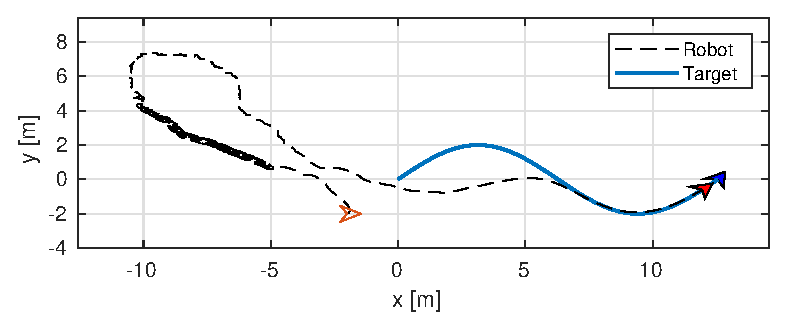
\includegraphics[width=0.48\textwidth,height=0.15\textheight]{matlabsim/sinePath/OUT/trajectorySineWave.eps} }
	\subfigure[][]{%    
    \label{fig:euclideanDistanceSin}%
    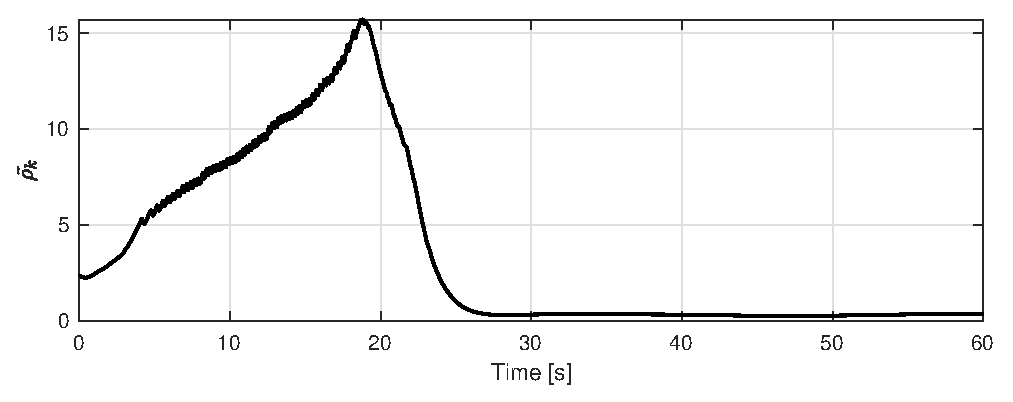
\includegraphics[width=0.48\textwidth,height=0.15\textheight]{matlabsim/sinePath/OUT/euclideanDistanceSineWave.eps} }
%  \\
%\subfigure[][]{%
%    \label{fig:stateErrorSin}%
%    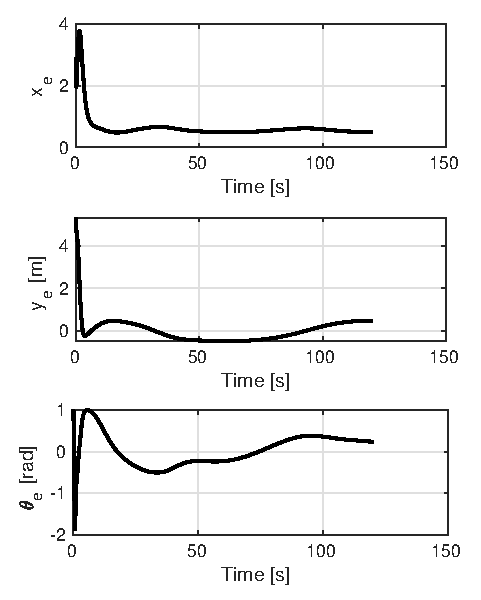
\includegraphics[width=0.48\textwidth,height=0.25\textheight]{figs/coppelia/secondScenario/stateErrorRandomPathDistance.eps} }
% \subfigure[][]{%
%    \label{fig:controlInputsSin}%
%    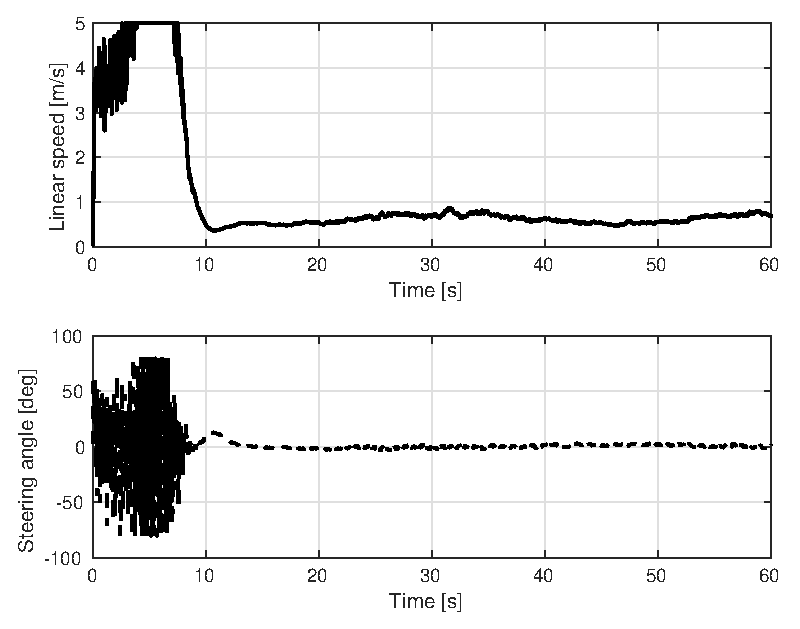
\includegraphics[width=0.48\textwidth,height=0.25\textheight]{figs/coppelia/secondScenario/controlInputRandomPathDistance.eps} }
  \\
 \subfigure[][]{%
    \label{fig:criticWeightSin}%
    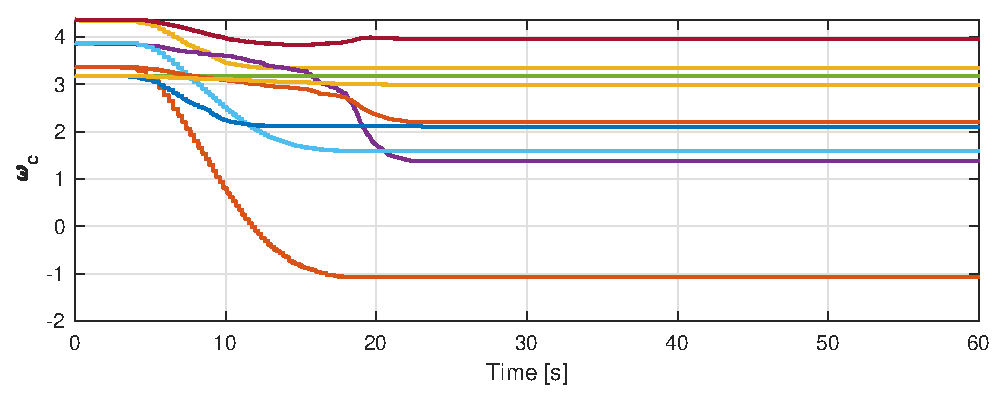
\includegraphics[width=0.48\textwidth,height=0.15\textheight]{matlabsim/sinePath/OUT/weightSineWave.eps} }
     \subfigure[][]{%
    \label{fig:actorWeightSin}%
    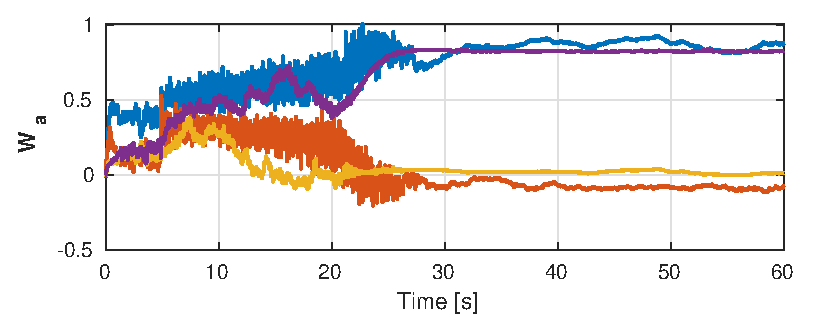
\includegraphics[width=0.48\textwidth,height=0.15\textheight]{matlabsim/sinePath/OUT/weightActorSineWave.eps} }
\caption[Robot tracking a target that is  following a sinusoidal trajectory.]{Robot tracking a target that is  following a sinusoidal trajectory:
  \subref{fig:trajectorySin} robot and target trajectories,~\subref{fig:euclideanDistanceSin} position error $\tilde\rho_k$, \subref{fig:criticWeightSin} critic learning weights~$\bm{\omega}_c,$ and \subref{fig:actorWeightRandom} actor learning weights~${\bf W}_a$}
    \label{fig:performanceSin}%
\end{figure*} 
%

In the second scenario, the target is set to move on a completely random trajectory starting from a random initial position $(x^{[d]},y^{[d]})\approx (2,-1)~[\si{\meter}],$ where the target is now modeled as a point robot as described in~\eqref{eq:leaderDT}
 %
where $\mathbf{u}_k^{[d]}=[\nu^{[d]},\omega^{[d]}] $ with
$\nu^{[d]}(t)=0.2~[\si{\meter}]$ and $\omega$ randomly changing in the range of
$({-\pi},{\pi}) $. The robot initial position and orientation are $(x,y) =
(0,0)~[\si{\meter}]$ and $\theta_0=0$. We intensify that the robot has no
previous knowledge of the dynamic model of the moving target. The results
obtained by the simulation are shown in Fig.~\ref{fig:performanceRandom}. Fig.~\ref{fig:trajectoryRandom} describes the trajectory of the robot and the target
during the simulation. The control actions of the robot are determined by the
random actor weights. We clearly see Euclidean distance in Fig.~\ref{fig:euclideanDistanceRandom} converges and approaches zero as actor and
critic weights converges to values that allows target tracking as can be seen in
Fig.~\ref{fig:criticWeightRandom}~and~\ref{fig:actorWeightRandom}. The results
reveal the ability of the proposed algorithm to successfully track the dynamic
moving target and adapt to the changes in the target's trajectory and learns
online by trial and error in different scenarios. %
%    
 \begin{figure*}[htbp]%
 \subfigure[][]{%
    \label{fig:trajectoryRandom}%
    \includegraphics[width=0.48\textwidth,height=0.15\textheight]{matlabsim/randomPath/OUT/trajectoryRandom.eps} }
	\subfigure[][]{%    
    \label{fig:euclideanDistanceRandom}%
    \includegraphics[width=0.48\textwidth,height=0.15\textheight]{matlabsim/randomPath/OUT/euclideanDistanceRandom.eps} }
%\subfigure[][]{%
%    \label{fig:stateErrorRandom}%
%    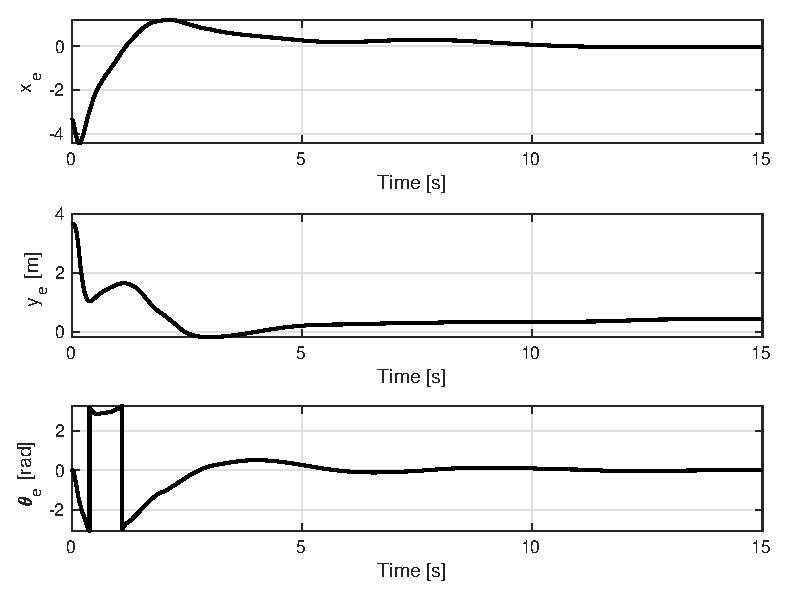
\includegraphics[width=0.48\textwidth,height=0.25\textheight]{figs/coppelia/firstScenario/stateErrorRandomPathDistance.eps} }
% \subfigure[][]{%
%    \label{fig:controlInputsRandom}%
%    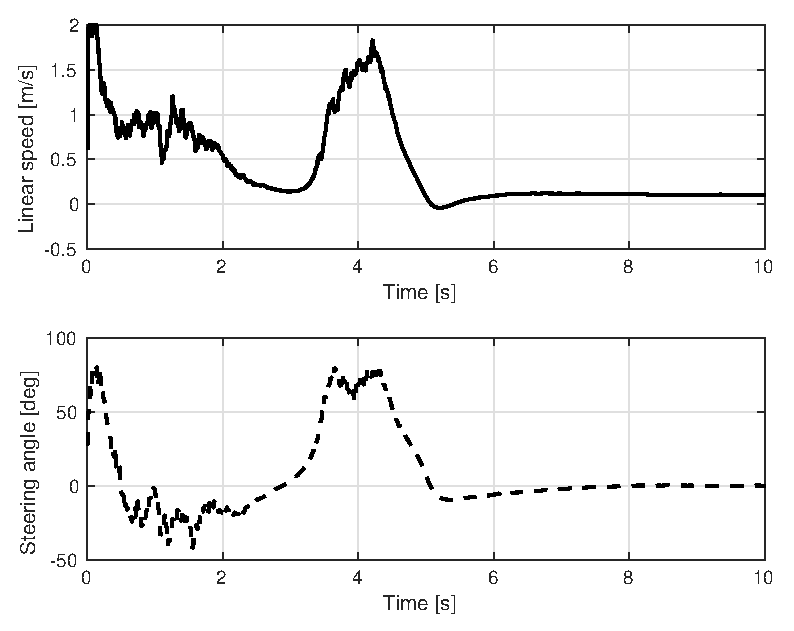
\includegraphics[width=0.48\textwidth,height=0.25\textheight]{figs/coppelia/firstScenario/controlInputRandomPathDistance.eps} }
 \subfigure[][]{%
    \label{fig:criticWeightRandom}%
    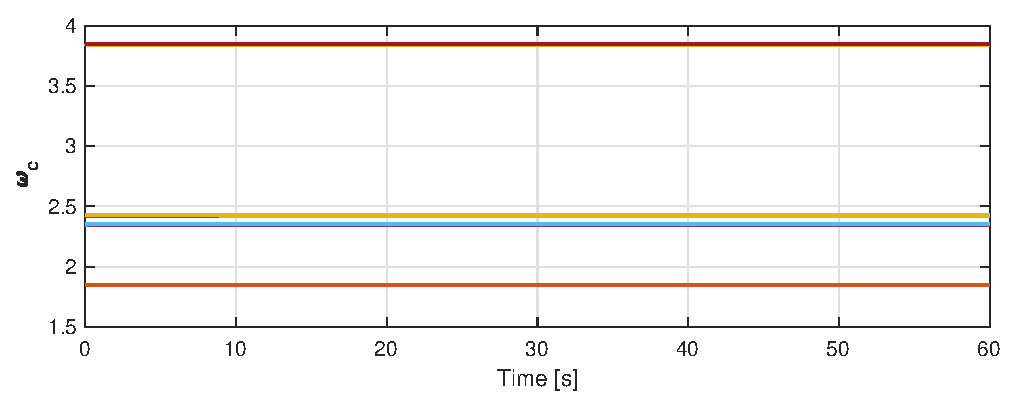
\includegraphics[width=0.48\textwidth,height=0.15\textheight]{matlabsim/randomPath/OUT/weightRandom.eps} }
     \subfigure[][]{%
    \label{fig:actorWeightRandom}%
    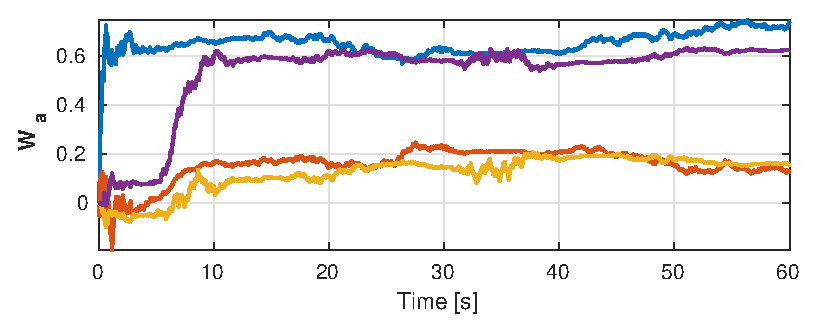
\includegraphics[width=0.48\textwidth,height=0.15\textheight]{matlabsim/randomPath/OUT/weightActorRandom.eps} }
  \caption[Robot tracking a target that is  following a random trajectory.]{Robot tracking a target that is  following a random trajectory:
  \subref{fig:trajectoryRandom} robot and target trajectories,~\subref{fig:euclideanDistanceRandom} position error $\tilde\rho_k$, \subref{fig:criticWeightRandom} critic learning weights~$\bm{\omega}_c,$ and \subref{fig:actorWeightRandom} actor learning weights~${\bf W}_a$}%
  \label{fig:performanceRandom}%
\end{figure*}


\section{Conclusion} \label{sec:conclusion}

A model free actor-critic reinforcement learning algorithm for dynamic target
tracking has been proposed and validated using a set of computer experiments  
where a differential drive mobile robot and a randomly moving target are
utilized in the simulation. As opposed to previous approaches in the literature,
the proposed approach possess the advantage of being completely model free and
does not  rely on any dynamic model of robots. The actor weights which
drives the control actions of the robot successfully converge to values that
enable the robot to asymptotically track the moving target through unplanned
trajectory. In future work, the proposed approach will be applied to multi-robot scenarios
where a number of robots are to achieve a certain task in unknown environments.
 


	\bibliographystyle{IEEEtran}
\bibliography{bib/refsSuruzWeb,bib/refsMultiAgent,bib/refsRoboticsJournals,bib/refsRoboticsConferences,bib/refsGenericControl,bib/refsBooksTRTheses,bib/refsReinforcementLearningADP,bib/refsRL-Keshtkar,bib/amrsRefs}
\end{document}

%%% Local Variables:
%%% mode: latex
%%% TeX-master: t
%%% End:
